% Live preprint. Hand-written text lives here and in sections/; every number, table and figure under generated/ is
% regenerated from experiment results by affdrift/reporting/paper.py (run after each scripts/aggregate.py).
\documentclass[10pt,twocolumn,letterpaper]{article}
\usepackage[pagenumbers]{cvpr}   % arXiv-style preprint: named authors, page numbers (template only; venue TBD)

\usepackage{iftex}
\ifXeTeX                          % tectonic builds with XeTeX: use a Times clone for the CVPR look
  \usepackage{fontspec}
  \setmainfont{texgyretermes}[Extension=.otf, UprightFont=*-regular, BoldFont=*-bold,
                              ItalicFont=*-italic, BoldItalicFont=*-bolditalic]
\fi
\usepackage{cuted}
\usepackage{caption}
\usepackage{multirow}
\usepackage{xcolor}
\newcommand{\pending}{\textcolor{gray}{[pending]}}
\newcommand{\affd}{AffD\xspace}
\newcommand{\Vp}{V^{+}}
\newcommand{\Vm}{V^{-}}
\newtheorem{lemma}{Lemma}
\newtheorem{proposition}{Proposition}

\definecolor{cvprblue}{rgb}{0.21,0.49,0.74}
\usepackage[pagebackref,breaklinks,colorlinks,allcolors=cvprblue]{hyperref}

% generated by affdrift/reporting/paper.py at 2026-11-08 13:49 UTC, commit 75d2109e82 — do not edit
\newcommand{\EOneThreeAffDCov}{$1$}
\newcommand{\EOneThreeAffDMCI}{$0.02572$}
\newcommand{\EOneThreeAffDMem}{$0.165$}
\newcommand{\EOneThreeAffDOff}{$0.279$}
\newcommand{\EOneThreeAffDRecall}{$0.94$}
\newcommand{\EOneThreeAffDW}{$0.469$ {\scriptsize$[0.46, 0.477]$}}
\newcommand{\EOneThreeDriftingMCI}{$1$}
\newcommand{\EOneThreeDriftingW}{$1.43$ {\scriptsize$[1.43, 1.43]$}}
\newcommand{\EOneThreeKOneMCI}{$0.9878$}
\newcommand{\EOneThreeKOneW}{$1.34$ {\scriptsize$[1.31, 1.36]$}}
\newcommand{\EOneThreeKThreeMCI}{$0.9996$}
\newcommand{\EOneThreeKThreeW}{$1.41$ {\scriptsize$[1.41, 1.42]$}}
\newcommand{\EOneThreeKTwoCov}{$1$}
\newcommand{\EOneThreeKTwoMCI}{$-0.2948$}
\newcommand{\EOneThreeKTwoMem}{$0.162$}
\newcommand{\EOneThreeKTwoOff}{$0.922$}
\newcommand{\EOneThreeKTwoW}{$1.06$ {\scriptsize$[1.06, 1.07]$}}
\newcommand{\EOneThreeRatio}{$0.33$}
\newcommand{\EOneThreeSingleCov}{$0.351$}
\newcommand{\EOneThreeSingleMCI}{$0.9996$}
\newcommand{\EOneThreeSingleMem}{$0.00443$}
\newcommand{\EOneThreeSingleOff}{$1$}
\newcommand{\EOneThreeSingleW}{$1.41$ {\scriptsize$[1.41, 1.42]$}}
\newcommand{\EOneTwoDriftingCov}{$0.339$}
\newcommand{\EOneTwoDriftingMCI}{$1$ {\scriptsize$[1, 1]$}}
\newcommand{\EOneTwoDriftingOff}{$1$}
\newcommand{\EOneTwoDriftingW}{$1.43$}
\newcommand{\EOneTwoOracleCov}{$0.977$}
\newcommand{\EOneTwoOracleMCI}{$0.09065$ {\scriptsize$[0.08467, 0.09446]$}}
\newcommand{\EOneTwoOracleOff}{$0.18$}
\newcommand{\EOneTwoOracleW}{$0.503$}
\newcommand{\EOneTwoSingleCov}{$0.351$}
\newcommand{\EOneTwoSingleMCI}{$0.9996$ {\scriptsize$[0.9995, 0.9997]$}}
\newcommand{\EOneTwoSingleOff}{$1$}
\newcommand{\EOneTwoSingleW}{$1.41$}
\newcommand{\EZeroFiveBMaxErr}{$3.3\times10^{-6}$}
\newcommand{\EZeroFiveLamQuarterErr}{$0.0278$}
\newcommand{\EZeroOneErr}{$1.6\times10^{-15}$}
\newcommand{\EZeroThreeDriftingSelf}{$0.951$}
\newcommand{\EZeroThreeSmoothTV}{$1.0\times10^{-4}$}
\newcommand{\EZeroThreeTV}{$0.147$ {\scriptsize$[0.145, 0.149]$}}
\newcommand{\GFourCFloor}{$0.0876$}
\newcommand{\GFourCW}{$0.136$ {\scriptsize$[0.129, 0.144]$}}
\newcommand{\VerdictEOneFive}{\pending{}}
\newcommand{\VerdictEOneFour}{\pending{}}
\newcommand{\VerdictEOneFourB}{\pending{}}
\newcommand{\VerdictEOneOne}{\textsc{pass}}
\newcommand{\VerdictEOneSix}{\pending{}}
\newcommand{\VerdictEOneThree}{\textsc{pass}}
\newcommand{\VerdictEOneTwo}{\textsc{pass}}
\newcommand{\VerdictEZeroFive}{\textsc{fail}}
\newcommand{\VerdictEZeroFiveB}{\textsc{pass}}
\newcommand{\VerdictEZeroFour}{\textsc{pass}}
\newcommand{\VerdictEZeroOne}{\textsc{pass}}
\newcommand{\VerdictEZeroSix}{\textsc{fail}}
\newcommand{\VerdictEZeroThree}{\textsc{fail}}
\newcommand{\VerdictEZeroTwo}{\textsc{inconclusive}}
\newcommand{\VerdictGFour}{\textsc{fail}}
\newcommand{\VerdictGFourB}{\textsc{fail}}
\newcommand{\VerdictGFourC}{\textsc{pass}}
\newcommand{\BuildStamp}{2026-11-08 13:49 UTC, commit \texttt{75d2109}}


\def\confName{CVPR}
\def\confYear{2027}

\title{Affinity Drifting: Learning Conditional Distributions\\from One Sample per Condition}

\author{Chan Lee\\
{\small Working draft --- results update automatically as experiments finish (\BuildStamp)}}

\begin{document}
\maketitle

\begin{abstract}
Drifting models train a one-step generator by moving its samples along a field that attracts them to data and repels
them from each other. In text-to-image data, however, each caption usually comes with a single image. We show that
with one positive per condition the attraction term reduces exactly to $L_2$ regression onto that positive, so a
generator that cannot resolve nearby conditions collapses to the conditional mean. We propose \emph{Affinity Drifting}
(\affd), which replaces the single target by a kernel mean-shift over the positives of semantically similar conditions,
weighted by a caption-space affinity. For Gaussian kernels the field is the gradient of a log density ratio, which
lets us predict its fixed points: borrowing positives with self-only repulsion converges to a Nadaraya--Watson mixture,
while symmetric repulsion memorises. We test this bottom-up with pre-registered, single-factor experiments. In a
non-parametric particle system the predicted fixed points are reached at the resolution of the kernel. In a 2-D toy
whose conditional distributions are known, the original Drifting objective and the single-positive objective both
collapse to the conditional mean (mean-collapse index \EOneTwoDriftingMCI\ and \EOneTwoSingleMCI), while an oracle with
many positives does not (\EOneTwoOracleMCI). Borrowing positives restores the mixture: \affd covers every mode and
lowers the held-out $W_2$ to \EOneThreeRatio\ of the single-positive objective, matching the oracle. Controls show why:
averaging the borrowed targets without the $x$-dependent kernel still collapses, and random instead of semantic
neighbours spread samples off the conditional manifold.
\end{abstract}

\begin{figure*}[t]
  \centering
  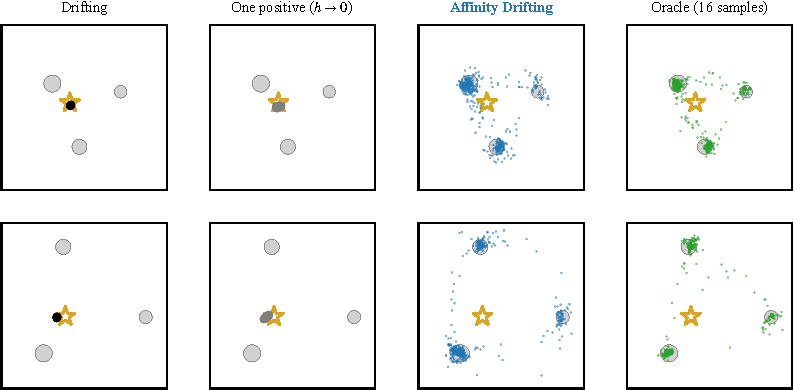
\includegraphics[width=\linewidth]{generated/figures/fig_teaser}
  \caption{\textbf{Mean collapse with one positive per condition.} Samples (512 per panel) from generators trained on a
  2-D toy where each training condition $c$ has exactly one sample, on two held-out conditions. Grey: true
  $p(x\mid c)$, a three-mode mixture; hollow $\star$: the conditional mean $\mathbb E[x\mid c]$. The original Drifting
  objective and the single-positive objective put every sample at the conditional mean, between the modes; an oracle
  given many true samples per condition covers the modes. \affd uses only the single positives, borrowed across similar
  conditions, and recovers the modes. Held-out conditions, seed 0 of five.}
  \label{fig:teaser}
\end{figure*}

\section{Introduction}
\label{sec:intro}

One-step generators trained by \emph{drifting}~\cite{deng2026drifting} evolve the pushforward of a noise distribution
during training rather than at sampling time: each generated sample is attracted toward data and repelled from the
other samples, and the generator regresses onto its own drifted outputs. With class labels, every class has many
images and the attraction is a proper mean-shift toward the class distribution.

Text conditioning breaks that assumption. A caption typically describes one image, so the positive set of a condition
has size one. Then the normalised attraction weight is one and the attraction no longer depends on where the sample
is: it is $L_2$ regression onto the single positive (Lemma~\ref{lem:regression}). A generator with finite resolution in
$c$ averages the positives of conditions it cannot tell apart and outputs their mean --- a blurred blob between modes
(\cref{fig:teaser}).

We ask whether \emph{borrowing} positives from semantically close conditions restores a distribution, and why. \affd
weighs every positive $y_i$ by a caption affinity $w_i(c)$ and keeps the $x$-dependent kernel of drifting, so the
attraction becomes a mean-shift toward a mixture rather than a pull toward an average. The claim is mechanistic: the
gain should come from the $x$-dependent mode assignment, not merely from having more targets. We therefore test it
with controls that remove each alternative explanation in turn --- averaging targets without $x$-dependence (K1),
random instead of semantic neighbours (K2), noise-smoothed single targets (K3) --- against an oracle with true samples
(K4) and the original Drifting objective as a baseline.

\paragraph{Contributions.} (i) The single-positive degeneracy of drifting and its consequence, mean collapse under
limited conditional capacity. (ii) \affd, with a fixed-point analysis for Gaussian kernels. (iii) A pre-registered,
single-factor experimental protocol, run bottom-up from particles to neural toys; this draft reports what is
finished and marks the rest as pending.

\section{Method}
\label{sec:method}

\paragraph{Drifting.} A generator $f_\theta(\epsilon, c)$ maps noise to samples. Given a field $V(x\mid c)$, it is
trained with $\mathcal L = \lVert f_\theta(\epsilon,c) - \mathrm{sg}(f_\theta(\epsilon,c) + V)\rVert^2$, where
$\mathrm{sg}$ stops the gradient. The field is attraction minus repulsion, $V = \Vp - \Vm$, each a kernel mean-shift:
\begin{equation}
  \Vp(x\mid c) = \frac{\sum_i w_i(c)\,k(x, y_i)\,(y_i - x)}{\sum_i w_i(c)\,k(x, y_i)},
  \label{eq:vplus}
\end{equation}
and $\Vm$ the same over the other generated samples. In the original method the positives are the samples of the
condition's own class, $w_i(c) = \mathbf{1}[c_i = c]$, and the field is normalised to unit energy per batch.

\begin{lemma}[Single positive is regression]\label{lem:regression}
If condition $c$ has one positive $y$ and repulsion is off, $\Vp(x\mid c) = y - x$ for every kernel, so
$\nabla_\theta\mathcal L = \nabla_\theta\lVert f_\theta - y\rVert^2$.
\end{lemma}

\paragraph{Affinity Drifting.} \affd keeps \eqref{eq:vplus} but borrows positives from similar conditions,
\begin{equation}
  w_i(c) = \exp\!\big(-\lVert\psi(c) - \psi(c_i)\rVert^2 / 2h_p(c)^2\big),
\end{equation}
with a frozen condition embedding $\psi$ (an oracle in the toy, a text encoder later). The bandwidth $h_p(c)$ is the
smallest value whose effective number of neighbours $N_\mathrm{eff} = (\sum_i w_i)^2/\sum_i w_i^2$ reaches $N^*=16$,
so every condition borrows equally strongly. Repulsion uses a caption bandwidth $h_q$; by default $h_q=0$, \ie a sample
is repelled only by the other samples of its own condition. The single-positive objective is the limit $h_p\to 0$ of
the same code; unconditional drifting is $h_p, h_q\to\infty$.

\paragraph{Fixed points.} For a Gaussian kernel of width $\sigma$, \eqref{eq:vplus} is a scaled score:
\begin{lemma}[Score ratio]\label{lem:score}
$V(x\mid c) = \sigma^2\nabla_x\big[\log\hat p(x\mid c) - \log\hat q(x\mid c)\big]$, where $\hat p = \sum_i w_i(c)\,
k_\sigma(\cdot, y_i)$ and $\hat q$ is the kernel density of the generated samples.
\end{lemma}
Hence $V\equiv 0$ exactly when $\hat q = \hat p$. With $h_q = 0$ the equilibrium of a condition is the
Nadaraya--Watson mixture of its borrowed positives,
$q_c = \sum_i \tilde w_i(c)\,\delta_{y_i}$ with $\tilde w = w/\sum w$ (Proposition~C in our plan); with symmetric
repulsion $h_q = h_p$ the mixing cancels on both sides and every condition memorises its own positive
(Proposition~A). The bandwidth $h_q$ thus selects the equilibrium.

\paragraph{Implementation choices.} We use a mixture of kernel widths, $\sigma\in\{0.071, 0.384, 2.07\}$ from the
$N^*$-th-nearest-neighbour distance to the median pairwise distance of the positives, summing one field per width;
each width satisfies Lemma~\ref{lem:score}, so the fixed point is unchanged. As in the original method, the
\emph{whole} field is normalised to unit energy per batch and per width. A per-term normalisation, which we first
used, keeps $\Vp$ and $\Vm$ at unit size even where both should vanish and flung a few percent of single-positive
samples far outside the data; we report it in \cref{sec:status}.

\section{Experiments}
\label{sec:experiments}

\paragraph{Protocol.} Every comparison changes one knob of a base configuration; a run refuses to start if its
configuration differs from the declared change. Predictions and falsification criteria are committed before any run,
and verdicts (pass / fail / inconclusive) are computed from those committed rules only. All arms share seeds
(five per experiment), probe inputs and the learning rate, which is fixed once on an unconditional run. Intervals are
95\% paired bootstrap CIs over seeds. Every experiment also trains the original Drifting objective, unchanged, as a
reference that is reported but not judged.

\subsection{Fixed points in a particle system}
\label{sec:l0}

Without a network, each of 32 conditions on a line owns 256 particles moved by $x \leftarrow x + \eta V(x\mid c)$, \ie
a generator of unlimited capacity, with one positive per condition. The field matches the autograd score ratio of
Lemma~\ref{lem:score} to \EZeroOneErr\ (float64; \VerdictEZeroOne). Increasing $h_q$ from $0$ to $h_p$ moves the
equilibrium monotonically from the mixture to memorisation (\cref{fig:l0}; \VerdictEZeroFour), whereas the original
Drifting objective memorises outright (own-positive share \EZeroThreeDriftingSelf).

\begin{figure*}[t]
  \centering
  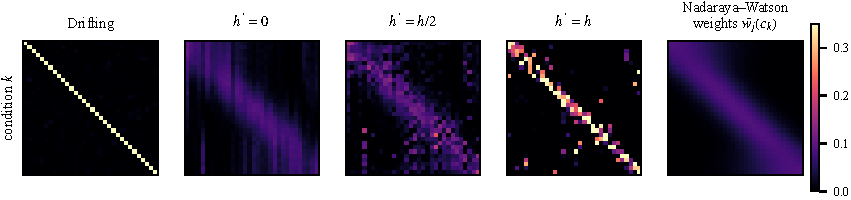
\includegraphics[width=\linewidth]{generated/figures/fig_l0}
  \caption{\textbf{$h_q$ selects the equilibrium} (particles, seed mean). Share of each condition's particles
  nearest to each positive. Original Drifting memorises (diagonal). \affd with $h_q=0$ spreads mass over the
  borrowed neighbours, as the Nadaraya--Watson weights $\tilde w$ predict (right); larger $h_q$ narrows the band
  toward memorisation.}
  \label{fig:l0}
\end{figure*}

The point-level assignment, however, misses the pre-registered tolerance for the mixture
(TV \EZeroThreeTV\ against $0.1$; \VerdictEZeroThree): with a kernel wider than the spacing of the positives, the
field cannot resolve which nearby positive a particle sits on. Compared at the kernel's resolution --- TV between the
$\sigma$-smoothed densities, an analysis we did not pre-register --- the equilibrium matches $\hat p$ to
\EZeroThreeSmoothTV. A counterfactual negative between two conditions has the predicted closed-form Gaussian
equilibrium in its algebra (relative error \EZeroFiveBMaxErr\ under a Gaussian closure), but with finite samples it is
stable only for small weights (error \EZeroFiveLamQuarterErr\ at $\lambda=0.25$, divergence from $\lambda=0.5$;
\VerdictEZeroFive).

\subsection{Mean collapse and its repair in a 2-D toy}
\label{sec:l1}

\paragraph{Setup.} Conditions $c\in[0,1]^2$ are drawn once; each of the $10{,}000$ training conditions has a single
positive from $p(x\mid c)$, a three-mode Gaussian mixture whose modes rotate with $c_1$ and whose radius and weights
change with $c_2$, so the conditional mean falls between modes. An MLP generator $f(\epsilon, g(c))$ sees $c$ quantised
to cells of width $\delta=1/16$, roughly 39 training conditions per cell. We train with Adam ($10^{-3}$, chosen on the
unconditional model: marginal $W_2$ \GFourCW\ against a sampling floor of \GFourCFloor), an EMA of the weights,
$20{,}000$ steps, and 8 conditions $\times$ 64 samples per batch, and evaluate on 256 held-out conditions with 512
samples each. The mean-collapse index is $\mathrm{MCI} = 1 - \operatorname{tr}\mathrm{Cov}_q/\operatorname{tr}\mathrm{Cov}_p$.

\paragraph{Single positive collapses (C1).} Both the original Drifting objective and the single-positive objective
collapse every condition to a point at the conditional mean (MCI \EOneTwoDriftingMCI\ and \EOneTwoSingleMCI;
off-manifold share \EOneTwoSingleOff), while the oracle with 16 true samples per condition and step covers the modes
(MCI \EOneTwoOracleMCI, mode coverage \EOneTwoOracleCov). This is the failure \affd targets
(\VerdictEOneTwo).

\begin{table}[t]
  \centering
  \small
  \resizebox{\linewidth}{!}{% generated — do not edit
\begin{tabular}{@{}lccccc@{}}
\toprule
Method & $W_2$ $\downarrow$ & $\operatorname{tr}\Sigma_q/\operatorname{tr}\Sigma_p$ & Prec. $\uparrow$ & Rec. $\uparrow$ & Modes $\uparrow$ \\
\midrule
Drifting & $1.4$ & $2.8\times10^{-5}$ & $0.0023$ & $0$ & $0.34$ \\
One positive ($h\to 0$) & $1.4$ & $3.8\times10^{-4}$ & $0.0017$ & $1.5\times10^{-6}$ & $0.35$ \\
Constant sample kernel & $1.3$ & $0.012$ & $0.0022$ & $0.007$ & $0.48$ \\
Random neighbors & $1.1$ & $1.3$ & $0.1$ & $0.97$ & $1$ \\
Noisy positive & $1.4$ & $4.4\times10^{-4}$ & $1.2\times10^{-5}$ & $0$ & $0.36$ \\
\midrule
\textbf{Affinity Drifting} & $0.47$ & $0.97$ & $0.74$ & $0.94$ & $1$ \\
Oracle (16 samples) & $0.5$ & $0.91$ & $0.83$ & $0.78$ & $0.98$ \\
\bottomrule
\end{tabular}
}
  \caption{\textbf{2-D toy, held-out conditions} (seed means). Above the line: the single-positive regime and the
  three mechanism controls; below: the oracle upper bound. [pending] entries fill in when E1.3 is aggregated.}
  \label{tab:l1}
\end{table}

\paragraph{Borrowing restores the mixture (C2).} \affd against the single-positive objective and controls K1--K3 is
\VerdictEOneThree\ (held-out $W_2$: \affd \EOneThreeAffDW, single \EOneThreeSingleW, ratio \EOneThreeRatio;
\cref{tab:l1}). \Cref{fig:mechanism} shows the mechanism: with one positive every attraction arrow points at the same
target, whereas the borrowed positives split the space into one basin per mode.

\begin{figure}[t]
  \centering
  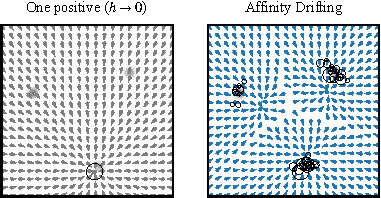
\includegraphics[width=\linewidth]{generated/figures/fig_mechanism}
  \caption{\textbf{Mechanism.} Direction of the attraction $\Vp(x\mid c)$ for one training condition. Single
  positive: every arrow points at the one target. \affd: arrows point to the nearest mode of the borrowed positives
  (circles, size $\propto$ weight).}
  \label{fig:mechanism}
\end{figure}

\paragraph{The gap grows with lost capacity (C3).} \VerdictEOneFour\ (\cref{fig:phase}).

\begin{figure}[t]
  \centering
  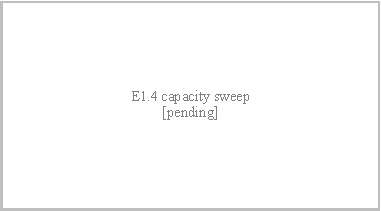
\includegraphics[width=\linewidth]{generated/figures/fig_phase}
  \caption{\textbf{Capacity.} $W_2$ of the single-positive objective and of \affd as the generator's resolution in
  $c$ coarsens (seed mean, 95\% CI).}
  \label{fig:phase}
\end{figure}

\section{Status, deviations and limitations}
\label{sec:status}

This is a working draft; \cref{tab:status} lists every pre-registered experiment and its outcome at the time of the
build. Changes to the plan are logged with reasons and approvals before any affected run; those that matter for
reading the results are the following. The learning-rate selection failed twice before passing: first because the
unconditional model was mis-specified (negatives from each condition's samples rather than from the whole batch), then
narrowly. A single kernel scale transported mass too locally and was replaced by three scales. 64 instead of 8 samples
per condition are generated, since negatives estimated from 8 samples are strongly biased. The drift normalization was
changed from separate normalization of $\Vp$ and $\Vm$ to normalization of the whole field, as
in~\cite{deng2026drifting}, after the separate version sent one-positive samples outside the data. Runs made before a
correction are kept and excluded from all results.

The toy uses the true condition coordinates as the embedding $\psi$; text embeddings, learned features and real
captions are later stages of the study and are not reported here.

\begin{table}[h]
  \centering
  \small
  \resizebox{\linewidth}{!}{% generated — do not edit
\begin{tabular}{@{}llll@{}}
\toprule
Level & ID & Claim & Verdict \\
\midrule
L0 & E0.1 & Lemma 1 & \textsc{pass} \\
L0 & E0.2 & Prop A & \textsc{inconclusive} \\
L0 & E0.3 & Prop C & \textsc{fail} \\
L0 & E0.4 & Prop A–C & \textsc{pass} \\
L0 & E0.5 & Prop E & \textsc{fail} \\
L0 & E0.5b & Prop E (diagnostic) & \textsc{pass} \\
L0 & E0.6 & Normalisation (cue 1) & \textsc{fail} \\
L1 & E1.1 & C0 & \textsc{pass} \\
L1 & E1.2 & C1 & \textsc{pass} \\
L1 & E1.3 & C2 & \textsc{pass} \\
L1 & E1.4b & C3 & \pending{} \\
L1 & E1.4 & C3 & \pending{} \\
L1 & E1.5 & C4 & \pending{} \\
L1 & E1.6 & Bandwidth selection & \pending{} \\
L1 & G4 & Gate G4 & \textsc{fail} \\
L1 & G4b & Gate G4 (2nd) & \textsc{fail} \\
L1 & G4c & Gate G4 (3rd) & \textsc{pass} \\
\bottomrule
\end{tabular}
}
  \caption{Pre-registered experiments and their outcomes at build time.}
  \label{tab:status}
\end{table}

\section{Related work}
\label{sec:related}

\affd builds on drifting~\cite{deng2026drifting}, which turns kernel mean-shift~\cite{comaniciu2002meanshift} into a
training signal for one-step generators. Its attraction is a Nadaraya--Watson kernel regression~\cite{nadaraya1964,
watson1964} over borrowed positives, and the field is closely related to gradients of kernel two-sample statistics
(MMD)~\cite{gretton2012kernel}, which generative models have used with mixtures of kernel widths for the same reason
we do~\cite{li2017mmdgan}. Our evaluation follows standard practice for mode collapse: precision and
recall~\cite{kynkaanniemi2019improved} and density and coverage~\cite{naeem2020reliable}. The capacity control by
spectral normalisation follows~\cite{miyato2018spectral}.


{
    \small
    \bibliographystyle{ieeenat_fullname}
    \bibliography{main}
}

\end{document}
